\chapter{Background and Analysis}
\section{Background}
In this section I will be talking about the Wizard Card Game, how the game works and how you can win the game and show in this video\cite{wizardVideo}. I will also discuss the Artificial Intelligence techniques that were consider using for the opponents, which are neural networks, minmax and Monte Carlo algorithms. This will be expanded upon to how I concluded using the Monte Carlo Tree search for this game.
\subsection{Wizard Card Game}
\subsubsection{Dealing and Setup}
Wizard is a card game that contains 52 normal deck cards and 8 extra cards 4 of which are called wizards and the other 4 are called jesters\cite{wizardOver}. Each player is dealt the same number of cards that is the round. For example, round 1 means each person get 1 card but round 10 means they each get ten cards. This is then played until the is no cards left to be dealt out mean for 3 people there should be 20 round and 15 rounds for 4 people. A trump card is also dealt from the deck at the beginning of the round from the top. After each play in a round the dealer is changed clockwise.
\subsubsection{Playing and Bidding}
One the trump has been dealt, the person to the left of the dealer states how many tricks they think they will win in this round. The maximum they can bid it the number of cards they have in their hands. Once everyone has put their individual bids in, the player to the left of the dealer puts down the first card which can be any card they want, then each player can either match the suit that the first player put down or the better play it to match the trump suit or play a wizard to win. Otherwise they can play off suit or play a jester to lose.
\subsubsection{Scoring}
To score points in this game you must use the bid on how many tricks you think you can win, giving you 20 point for being right and 10 point for every trick you win. Otherwise you get negative 10 point per every trick you were over or under for that round. For example, if you guess 4 tricks to win and only one 1 you would lose 30 points. 

\subsection {Monte Carlo Algorithm}
The Monte Carlo Algorithm is probabilistic search algorithm that creates a tree based on the current states of the problem. This is then randomly expanded from the root node and simulated what might happen, under specific constrains such a iterations of the simulation or under an amount time. This will then give a score back on what how well the simulation wen. once this is done the best option will be picked based on what has the highest score from the tree that has currently been created. The next sections below will show the 4 phases that are used in the algorithm.
\begin{figure}[h]
\centering
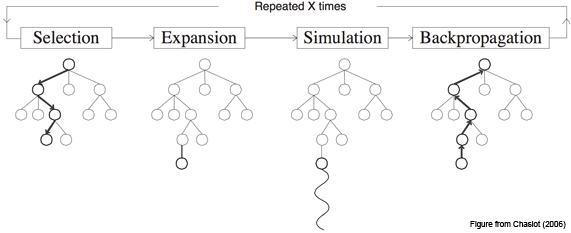
\includegraphics[width=15cm]{mcts-algorithm-1a}
\caption{Diagram Showing Steps in Monte Carlo Tree Search}
\end{figure}[h]
\subsubsection{Selection}
For this phase in the algorithms it will start with the root node that shows the initial state of the game. This will then select the child node that has the best win rating. this win rating will be selected by the use if Uct(Upper Confidence Bound for Trees). The formula used for this is:

\begin{itemize}
\item w\textsubscript{i} : This variable will contain the number of wins the node will have after \textit{i} amount of moves.
\item n\textsubscript{i} : This is the number of simulation after the \textit{i} amount of moves
\item c : This is this exploration parameter and should theoretically be equal to .
\item t : the total number of simulations performs for the parent node.
\cite{mctswithcode}
\end{itemize}
\subsubsection{Expansion}
After the selection of a node is complete we do the expansion of this node. This is done by adding a new child node to the tree that was optimally reached during the selection process\cite{mctsSource}.
\subsubsection{Simulation}
Once the node has been expanded ,we perform a simulation of the state until it reach the end of what we are trying to achieve. For example in the project we would simulate the selection of the cards until there are non left and how large there score is.
\subsubsection{Backpropagation}
In this part of the process we look at the result of the simulation and give a reward for how good the simulation was. In the context of this game the close the score is to the initial bid the better it is, meaning that we shall reward the child node with a higher score the larger the score and closer to the bid.


Once this is done under it will be repeat for a set number of iterations or under a specific time period. This will then create an asymmetric search tree that grows after each iteration through the steps. Once it is done iterating, it will pick the best child node best on the best score divided by the number of visits that specific node has.
\subsubsection{Advantages}
\begin{itemize}
\item Compared to other AI algorithms this is quite a simple algorithm to implement.
\item As this is a heuristic algorithm is does not need to everything that happens in the game apart from the rules of the game, how it ends the simulation/leaf node and what cards the player may have. this is because it can find it own moves and randomly playout the game.
\item The tree that has been creates can be used for the future meaning less computational expense creating more nodes.
\item As you can select the number of iterations/time given, it means you can make the tree as small or large as you would like. 
\end{itemize}
\subsubsection{Disadvantages}
\begin{itemize}
\item The larger the tree growths the more rapidly memory expensive.
\item The algorithm normally needs a large amount of iteration to be able to effectively pick the best path, meaning that it will have to take amount of time to construct a large enough search space.
\end{itemize}

\subsection{Similar Algorithms}
In this section, I will be talking about the two other Algorithms that could have been used for the Artificial intelligence of the game. Discussion on why they was not used and why the Monte Carlo Tree Search was the one to be picked will also be talked about.
\subsubsection{Neural Network}
Neural Network are artificially created based on the neuronal structure of the mammalian cerebral cortex but on much smaller scales.\cite{NeuralNetwork}
\subsubsection{MinMax}


\section{Analysis}
In this section I will be talking about what I will be aiming doing achieve with this product and what technology I will be using during this process. 
\subsection{Project Aims}
The aim for this project is create a functional software version of the card game Wizard. This will also contain an Artificial intelligence Opponent that uses the Monte Carlo Algorithm to select a card for that round. The game will be simplified to only have 3 players, two of which will be the AI and one which is the human player. Each player will have 15 cards each and play until there are no cards left for 5 rounds.
\begin{figure}[h]
\centering
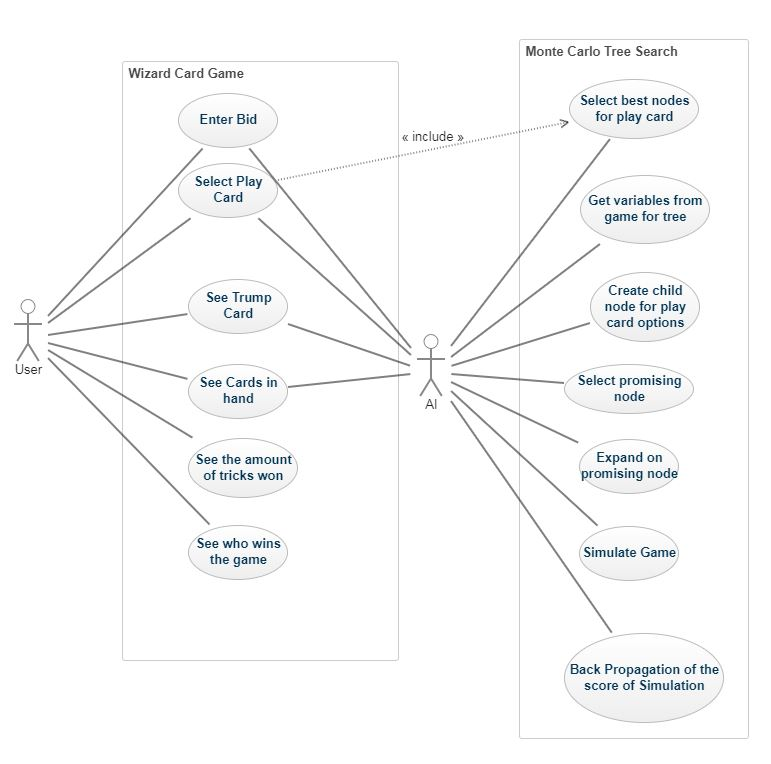
\includegraphics[width=15cm]{Wizard_UML}
\caption{Diagram Showing the Use Case for the Project}
\end{figure}[h]
Below shows the descriptions of the different use cases:
\begin{itemize}
\item Enter bid - A bid must be selected based on what cards are in the players hands for what score they think they will get.
\item Select Play Card - A play card must be selected based on what the trump card is, what the other players have player and what cards the player has to use.
\item See Trump Card - Printing of the Trump card so that a selection of the play card can be made and see if it is valid card to play.
\item See Cards in hand - Print the cards that are currently in the hand of the player so a card can be selected from that hand.
\item See the amount of trick won - Show the number of tricks that they have won at the end of the round so they can see how close it was to their bid.
\item See who wins the game - To show who won overall in the game
\item Select best nodes for play card - Select the node with the largest score to visit ratio and play the card in the game for that player.
\item Get Variables from game to tree - Gets all the variables needed to create the tree such as the cards in the players hand and what the trump card is.
\item Create child node for play card options - Create child nodes from the current game state that contain the possible moves played by the players.
\item Select promising node - Selects a node to explore to see simulate and see how good of an option it is.
\item Expand on promising node - Expands on the node it is currently exploring the make the tree and only stops after it cannot expand any more.
\item Simulate Game - Simulate the game to show the what may happen in the game and see if it is a good option.
item Back Propagation of the score of Simulation - Gives a score to the child of the root node based on how good the simulation was and how many times that node was visited.
\end{itemize}
\subsection {Technology Overview}
This section will contain information on the technologies that are used in the project and how the help to achieve the goals that have been set.
\subsubsection{Programming Language and Software}
The programming language used for the project is was java\cite{javadescript} and the IDE for to implement it was IntelliJ IDEA 2018, this was because of the experience in using this language made it a better option than the others. As Java is an object oriented programming language, it makes it easier for changes to the program in the future for different type of AI that could be used or implemented for the Wizard card game\cite{java}. As this was more focus on the AI aspect of the game the fact that java atomically allocates and has garage collection made it easier to focus on making the AI. As for the IDE, it was chosen for the easy of use for java and in the way in which the debugging works will make it easier to find problems with the program. 

Another project that will be use in the project will be TeXworks\cite{tex} using the Latex to produce a pdf, which is a word processors for the development of the project report. This was chosen as it may be more difficult to initially write with over another processor such as Microsoft Word but as there is some experience in the use of it, using it can produce a better document and can be quicker to produce with such functions as the automated content page being produces as you develop \cite{Latex}. using latex makes it easier to separate out different sections of works without having the completely changing everything. 
\subsubsection{Hardware}
As this project doesn’t require a large amount of data space or processing speed to function, simple hardware would suffice in it usage. However a large amount of memory would be useful for large amount of iterations in the tree search. The hardware that will be used the build the software is:
\begin{itemize}
\item Processor: Intel(R) Core(TM) i7-7700HQ @ 2.80GHz
\item Installed Memory(RAM): 16.00 GB
\item System Type: 64-bit Operating System
\item: Operating System: Windows 10 Home
\end{itemize} 
With the hardware that is being used, there is ample memory to give the tree search a large number for testing and then reduce it for a more standard amount of memory.
\section{Research Method and Software Process}
\subsection {Foreseen Challenges}
One of the challenges that will be faced during the project will be making sure that the all of the rules of the game are applied and that all of the player within the game will follow it. Another problem that will arise will be trying to implement the Monte Carlo Tree Search as a lot if the reference are for two player games meaning it will have to be manipulated to work for the game. Deciding on how to score what it the best simulation will also be difficult as it will depend on how close they are to the bid or how many tricks the players win.
applying Rules, Implementing Mont Carlo Tree search and optimising.
\subsection {Process Methodology}
There was a lot of options for developing my project. In the end I decide to you a agile approach based on Scrum. This would give me an iterative way of progressing in the project, use the sprints in the methodology to progressively improve on the previous work that I have done, adding more functionality and complexity to it as it is being developed. This led to the conclusion that it was a better option then traditional methods such as the waterfall model. This is because the work can start on the software whilst writing up the report without having to do redo all the work that has previously done when changes are made to the design of the software.
\subsubsection{Version Control}
The version control during the development of this project will control use Git. This will be using a private GitLab repository of which my project will be stored in. The repository will allow me to back up my code regular and manage it. This would mean it could get back to a previous implementation of my code if there later version has broken. This will also be using this for my latex documentation which will also abide by these rules. As GitLab is externally hosted, it will be easily recoverable if there is a failure in the local storage.
